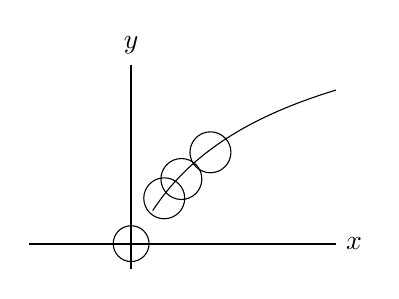
\begin{tikzpicture}[scale=0.65]
%axis
\draw[thick] (-2,0)--(4,0) node[right]{$x$};
\draw[thick] (0,-0.5)--(0,3.5) node[above]{$y$};

\draw[shorten <= 0.5cm] (0,0) to [bend left = 20] node[pos = 0.2] (N1) {} node[pos = 0.3] (N2) {} node[pos = 0.46] (N3) {} (4,3);
\foreach \x in {1, 2, 3}
    \draw (N\x) circle[radius = 0.4cm];


\draw (0,0) circle[radius = 0.35cm];

\end{tikzpicture}